\subsubsection*{Hyperparameters}

Hyperparameters for RDD2020 dataset: \texttt{SSD/configs/train\_rdd2020.yaml}.

Hyperparameters for TDT4265 dataset: \texttt{SSD/configs/train\_tdt4265.yaml}.

\subsubsection*{Running the code}
\emph{NB: Make sure you're in the \texttt{SSD/} directory.}

\underline{Training on the RDD2020 dataset:}

\texttt{python3 train.py configs/train\_rdd2020.yaml}

\underline{Training on the TDT4245 dataset:}

If you want to use a network pre-trained on the RDD2020 dataset, you must give a path to the \texttt{.pth} file that contains its parameters. In the config, set \texttt{PRETRAINED\_PATH} to this path. If you want to train from scratch, just remove \texttt{PRETRAINED\_PATH} from the config.

\texttt{python3 train.py configs/train\_tdt4265.yaml}


\subsubsection*{Network layout}

ResNet uses blocks to build up each layer. A block in ResNet18,
$
\begin{bmatrix}
  \texttt{filter size, channel} \\
  \texttt{filter size, channel}
\end{bmatrix},
$
is made up of two convolutions with filters of size $\texttt{filter size}$ and with output channels $\texttt{channel}$. There is batch normalization after each convolution, and the first convolution has a stride of 2, while the second has a stride of 1. There is a ReLU after the first convolution, and again after the skip connection $F(x)+x$. The network layout is shown in \cref{tab:layout}, where the last 6 layers are used as feature maps for SSD. In layer \texttt{Extra4}, the first convolution has a stride of 3, so that the size of the last feature map is $1\times1$.

\begin{table}[h!]
    \centering
    \begin{tabular}{|c|c|}
      \hline
      Layer name &  \\
      \hline
      Conv1 & \makecell{7$\times$7 filter, 64 channels, stride 2 \\ 3$\times$3 maxpool, stride 2} \\
      \hline
      \makecell{\rule{0pt}{4ex}Conv2\\\rule{0pt}{2ex}}& \makecell{$\begin{bmatrix} 3\times3, 64 \\ 3\times3, 64 \end{bmatrix}\times 2$}\\
      \hline
      \makecell{\rule{0pt}{4ex}Conv3\\\rule{0pt}{2ex}} & \makecell{$\begin{bmatrix} 3\times3, 128 \\ 3\times3, 128 \end{bmatrix}\times 2$}\\
      \hline
      \makecell{\rule{0pt}{4ex}Conv4\\\rule{0pt}{2ex}} & \makecell{$\begin{bmatrix} 3\times3, 256 \\ 3\times3, 256 \end{bmatrix}\times 2$}\\
      \hline
      \makecell{\rule{0pt}{4ex}Conv5\\\rule{0pt}{2ex}} & \makecell{$\begin{bmatrix} 3\times3, 512 \\ 3\times3, 512 \end{bmatrix}\times 2$}\\
      \hline
      \makecell{\rule{0pt}{4ex}Extra1\\\rule{0pt}{2ex}} & \makecell{$\begin{bmatrix} 3\times3, 512 \\ 3\times3, 512 \end{bmatrix}\times 2$}\\
      \hline
      \makecell{\rule{0pt}{4ex}Extra2\\\rule{0pt}{2ex}} & \makecell{$\begin{bmatrix} 3\times3, 512 \\ 3\times3, 512 \end{bmatrix}\times 2$}\\
      \hline
      \makecell{\rule{0pt}{4ex}Extra3\\\rule{0pt}{2ex}} & \makecell{$\begin{bmatrix} 3\times3, 512 \\ 3\times3, 512 \end{bmatrix}\times 2$}\\
      \hline
      \makecell{\rule{0pt}{4ex}Extra4\\\rule{0pt}{2ex}} & \makecell{$\begin{bmatrix} 3\times3, 512 \\ 3\times3, 512 \end{bmatrix}\times 2$}\\
      \hline
    \end{tabular}
    \caption{Network layout for both RDD2020 and TDT4265 datasets.}
    \label{tab:layout}
\end{table}


\subsubsection*{Model development requirements}

The fulfillment of the requirements listed in the project description should be clear from the code and config files.

\begin{itemize}
  \item The models use image sizes greater than $300\times 300$, as seen from both config files 
  \item The model for RDD2020 is a pre-trained ResNet, as seen from \texttt{resnet\_rdd.py} in the \texttt{backbone}.
  \item Only random horizontal mirror was used in the final models, but random sample crop was also tested. This can be seen from \texttt{\_\_init\_\_.py} in \texttt{transforms}, also shown in \figref{fig:transforms}.
\end{itemize}

\begin{figure}
  \centering
  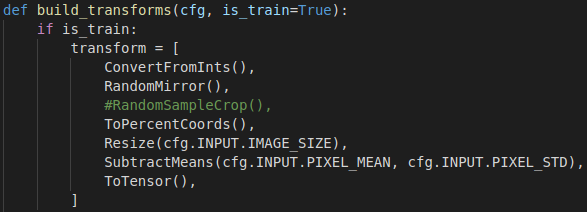
\includegraphics[width=\textwidth]{transforms.png}
  \caption{Transforms used in \texttt{\_\_init\_\_.py}.}
  \label{fig:transforms}
\end{figure}

